%\title{Using the forest package to create trees in LaTeX}
% From http://tex.stackexchange.com/a/108728/23931 
\documentclass[12pt,preview,border=0]{standalone}
\usepackage[paperheight=20cm,paperwidth=11cm]{geometry}
\usepackage{graphicx}
% \usepackage{forest}
\usepackage{amsmath}
% \usepackage{txfonts}  %pretty math font
\usepackage{kmath,kerkis}
\usepackage{tikz}
\usetikzlibrary{arrows,automata,positioning}

% \usepackage{fontspec}
% \defaultfontfeatures{Mapping=tex-text}
% \setmainfont[Scale=1,Ligatures={Common}]{Adobe Caslon Pro}
% \setromanfont[Scale=1,Ligatures={Common}]{Adobe Caslon Pro}
% \setmathrm[Scale=1]{Adobe Caslon Pro}
%\setmathfont(Digits,Latin)[Numbers={Lining,Proportional}]{Adobe Caslon Pro}


\begin{document} \begin{center}
		
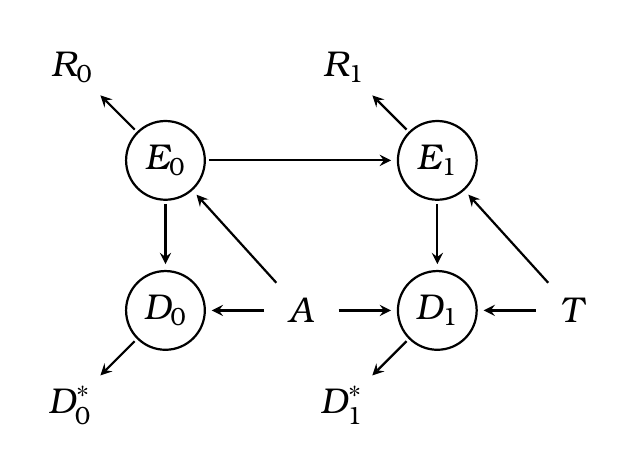
\begin{tikzpicture}[
	> = stealth, % arrow head style
	shorten > = 1pt, % don't touch arrow head to node
	auto,
	node distance = 2cm, % distance between nodes
	thick, % line style
	U/.style={circle, draw=black, inner sep=1.8pt, outer sep=1.5pt, minimum size=10mm, font=\Large},  %draw=black, fill=white
	O/.style={circle, inner sep=3.4pt, outer sep=-.75pt, minimum size=10mm, font=\Large},              %draw=white, fill=white
	]
	
	% Nodes and their relative positions
	% t = 0
   	\node[U] (E0) {$E_0$};
    \node[U] (D0) [below = .8 of E0] {$D_0$};	

    \node[O] (A) [right = .7 of D0] {$A$};
	\node[O] (R0) [above left = .65 of E0] {$R_0$};
   	\node[O] (DD0) [below left = .65 of D0] {$D_0^\ast$};
    % t = 1
    \node[U] (D1) [right = .7 of A] {$D_1$};	
    \node[U] (E1) [above = .8 of D1] {$E_1$};
    \node[O] (R1) [above left = .65 of E1] {$R_1$};
   	\node[O] (DD1) [below left = .65 of D1] {$D_1^\ast$};
   	\node[O] (T) [right = .7 of D1] {$T$};
       
	% Paths connecting nodes
    \path[->] (T) edge (D1);
    \path[->] (T) edge (E1);
    
    \path[->] (E1) edge (R1);
    \path[->] (E1) edge (D1);
    
    \path[->] (A) edge (D1);
    \path[->] (A) edge (D0);
    \path[->] (A) edge (E0);
    \path[->] (E0) edge (D0);
    \path[->] (E0) edge (R0);
    \path[->] (E0) edge (E1);
    
    \path[->] (D0) edge (DD0);
    \path[->] (D1) edge (DD1);
\end{tikzpicture}
	

\end{center}\end{document}
